\section{Fluid-Structure Interaction between an elastic object and laminar incompressible flow} \label{sec:HronTurek}
The goal of this benchmark is to test the fluid and solid solver first separately and then together as a full FSI problem \cite{Hron2006a}. This benchmark is based on the older benchmark " flow around cylinder" with fluid considered incompressible and in the laminar regime where the structure deformations are significant. The problem is setup with the solid submerged in the fluid, so that oscillations in the fluid deform the structure. We will measure the drag and lift around the circle and bar, and measure structural displacement at a given point. This benchmark will be used to test and verify different numerical methods and code implementations. Testing robustness and efficiency. 


\subsection{Problem Defintion}
\subsubsection*{Domain}

\begin{center}
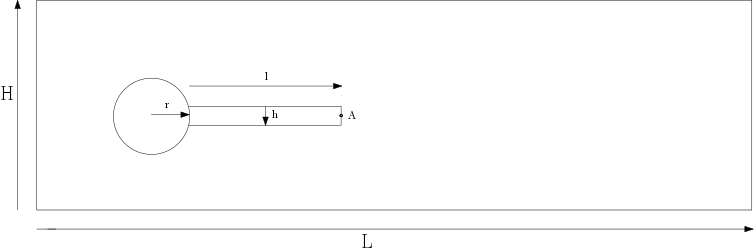
\includegraphics[scale=0.4]{./Verification_Validation/Hron_Turek/Domain_drawing.png}
\end{center}

The computational domain consists of a circle with an elastic bar behind the circle. The circle is positioned at (0.2, 0.2) making it 0.05 of center from bottom to top, this is done to induce oscillations to an otherwise laminar flow. 
This gives a force to the elastic bar. The parameters of the domain are:\\
L = 2.5, H = 0.41, l = 0.35, h = 0.02, A = (0.2, 0.6) \\

\subsubsection*{Boundary conditions}
The fluid velocity has a parabolic profile on the inlet that changes over time:\\

\begin{align*}
u(0,y) &= 1.5u_0 \frac{y(H-y)}{(\frac{H}{2})^2}  \\
u(0,y,t) &= u(0,y)\frac{1-cos(\frac{\pi}{2}t)}{2} \text{  for  } t<2.0 \\
u(0,y,t) &= u(0,y) \text{  for  } t \leq 2.0
\end{align*}

We set no slip on the "floor" and "ceiling" so to speak.\\
$$ u(x,y,t) = 0 \text{  on  } \partial \mathcal{F}_{floor and ceiling} $$
$$  p(x,y,t) = 0 \text{  on  } \partial \mathcal{F}_{outlet} $$

\subsubsection*{Quantities for comparison}
When the fluid moves around the circle and bar it exerts a force. These are split into drag and lift and calculated as follows:
$$ (F_d, F_L) = \int_S \sigma_f n dS $$ 
where S is the part of the circle and bar in contact with the fluid. \\
We set a point A on the right side of the bar. This point is used to track the deformation in CSM and FSI tests. \\
In the unsteady time dependent problems the values are represented with a mean , amplitude and frequency:
\begin{align}
mean =& \frac{1}{2} (max + min) \\
amplitude =& \frac{1}{2} (max - min)\\
frequency =& \frac{1}{T}
\end{align}

In each test the numbers with ref are the values taken from the benchmark paper \cite{Hron2006a}

\subsection{Results}
\subsubsection{CFD test}
The first two CFD tests are run with Reynolds number 20 and 100 giving steady drag and lift around the circle. CFD 3 has a Reynolds number 200 which will induce oscillations behind the circle, giving fluctuations in the drag and lift.
The CFD tests were run using the the bar as rigid object, that is the domain calculated is just the fluid domain. It is possible to also calculate with the bar and setting $\rho_s$ and $\mu_s$ to a large value. 

\begin{figure}[H]
\caption{Fluid mesh}
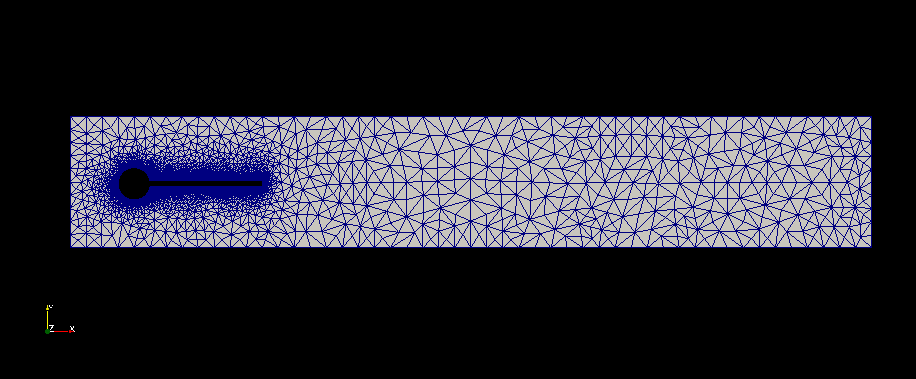
\includegraphics[scale=0.5,trim={24mm 46mm 14mm 40mm},clip]{./Verification_Validation/Hron_Turek/fluid.png}
\end{figure}

\vspace{1cm}

\begin{table}[H]
\centering
\caption{CFD parameters}
\label{my-label}
\begin{tabular}{|l|l|l|l|}
\hline
Parameters & CFD1 & CFD2 & CFD3 \\ \hline
$\rho_f [10^3 \frac{kg}{m^3}]$ & 1 & 1 & 1 \\ \hline
$\nu_f [10^{-3} \frac{m^2}{s}]$ & 1 & 1 & 1 \\ \hline
$ U [\frac{m}{s}] $ & 0.2 & 1 & 2 \\ \hline
Re = $\frac{Ud}{\nu_f}$ & 20 & 100 & 200 \\ \hline
\end{tabular}
\end{table}

\begin{table}[H]
\centering
\caption{CFD 1}
\label{my-label}
\begin{tabular}{|l|l|l|l|}
\hline
\textbf{elements} & \textbf{dofs} & \textbf{Drag} & \textbf{Lift} \\ \hline
6616 & 32472 & 14.2439 & 1.0869 \\ \hline
26464 & 124488 & 14.2646 & 1.11085 \\ \hline
105856 & 487152 & 14.2755 & 1.11795 \\ \hline
\textbf{ref} & \textbf{} & \textbf{14.29} & \textbf{1.119} \\ \hline
\end{tabular}
\end{table}

\begin{table}[H]
\centering
\caption{CFD 2}
\label{my-label}
\begin{tabular}{|l|l|l|l|}
\hline
\textbf{elements} & \textbf{dofs} & \textbf{Drag} & \textbf{Lift} \\ \hline
6616 & 32472 & 135.465 & 6.27158 \\ \hline
26464 & 124488 & 136.566 & 9.82166 \\ \hline
105856 & 487152 & 136.573 & 10.4441 \\ \hline
\textbf{ref} & \textbf{} & \textbf{136.7} & \textbf{10.53} \\ \hline
\end{tabular}
\end{table}

\subsubsection{CSM test}
The CSM test are calculated using only the bar and adding a gravity term $g$ with the same value but changing the parameters of solid. The tests CSM1 and CSM2 are steady state solutions. The difference is a more slender bar. The CSM 3 test is unsteady and even more slender causing the bar to move up and down. Since there is no resistance from any fluid the unsteady test should if energy is preserved make the bar move up and down infinitely. 

Our quantity for comparing there will be the deformation at the point $A$. 
\begin{center}
\begin{figure}[H]
\caption{Structure mesh}
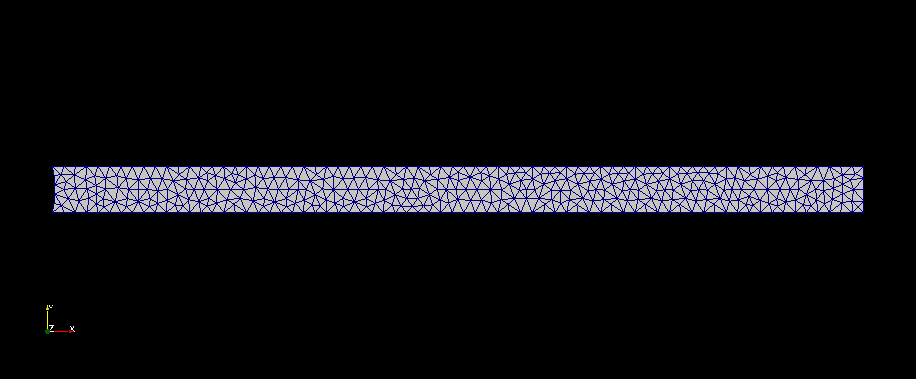
\includegraphics[scale=0.50,trim={18mm 55mm 18mm 55mm},clip]{./Verification_Validation/Hron_Turek/structure.png}
\end{figure}
\end{center}

\vspace{0cm}

\begin{table}[H]
\centering
\caption{Parameters}
\label{my-label}
\begin{tabular}{|l|l|l|l|}
\hline
Parameters & CSM1 & CSM2 & CSM3 \\ \hline
$\rho_f[10^3 \frac{kg}{m^3}]$ & 1 & 1 & 1 \\ \hline
$\nu_f [10^{-3} \frac{m^2}{s}]$ & 1 & 1 & 1 \\ \hline
$u_0$ & 0 & 0 & 0 \\ \hline
$\rho_s[10^3 \frac{kg}{m^3}]$ & 1 & 1 & 1 \\ \hline
$\nu_s$ & 0.4 & 0.4 & 0.4 \\ \hline
$\mu_s[10^6 \frac{m^2}{s}]$ & 0.5 & 2.0 & 0.5 \\ \hline
$g $ & 2 & 2 & 2 \\ \hline
\end{tabular}
\end{table}

\begin{table}[H]
\centering
\caption{CSM 1}
\label{my-label}
\begin{tabular}{|l|l|l|l|}
\hline
elements & dofs & $d_x(A) [\times10^{-3}]$ & $d_y(A) [\times10^{-3}]$ \\ \hline
725 & 1756 & -5.809 & -59.47 \\ \hline
2900 & 6408 & -6.779 & -64.21 \\ \hline
11600 & 24412 & -7.085 & -65.63 \\ \hline
46400 & 95220 & -7.116 & -65.74 \\ \hline
\textbf{ref} & \textbf{ref} & \textbf{-7.187} &  \textbf{-66.10} \\ \hline
\end{tabular}
\end{table}

\begin{table}[H]
\centering
\caption{CSM 2}
\label{my-label}
\begin{tabular}{@{}|l|l|l|l|@{}}
\hline
Elements & Dofs & $d_x(A) [\times10^{-3}] $& $d_y(A) [\times10^{-3}] $\\ \hline
725 &  1756 & -0.375 & -15.19 \\ \hline
2900 & 6408 & -0.441 & -16.46\\ \hline
11600 & 24412 & -0.462 & -16.84 \\ \hline
46400 & 95220 & -0.464 & -16.87\\ \hline
\textbf{ref} & \textbf{ref} &  \textbf{-0.469} &  \textbf{-16.97} \\ \hline
\end{tabular}
\end{table}

\begin{table}[H]
\centering
\caption{CSM 3}
\label{my-label}
\begin{tabular}{|l|l|l|l|}
\hline
elements & dofs & $d_x(A) [\times10^{-3}]$ & $d_y(A)[\times10^{-3}]$ \\ \hline
725 & 1756 & $-11.743 \pm 11.744$ & $-57.952 \pm 58.940$ \\ \hline
2900 & 6408 & $-13.558 \pm 13.559$ & $ -61.968 \pm  63.440 $ \\ \hline
11600 & 24412 & $ -14.128 \pm 14.127$ & $-63.216 \pm 64.744 $ \\ \hline
46400 & 95220 & $ -14.182 \pm 14.181 $ & $ -63.305 \pm 64.843 $ \\ \hline
\textbf{ref} &  & $ \textbf{-14.305} \pm \textbf{14.305} $ & $ \textbf{-63.607} \pm  \textbf{65.160} $ \\ \hline
\end{tabular}
\end{table}


\begin{figure}[H]  \label{CSM3_plots} 
  \caption {Displacement of point A, CSM3}
  \begin{minipage}[b]{0.5\linewidth}
    \centering
    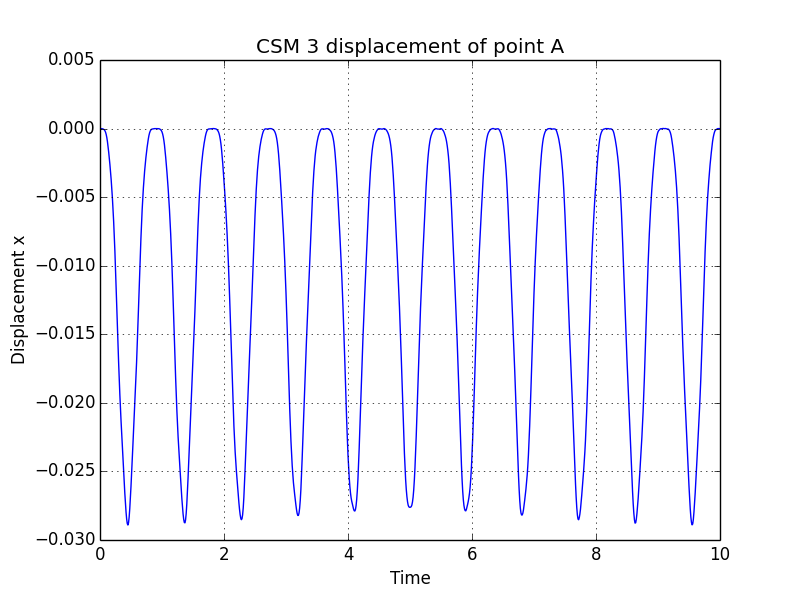
\includegraphics[width=.75\linewidth]{./Verification_Validation//Hron_Turek/dis_x.png} 
    \caption{Displacement x} 
    \vspace{4ex}
  \end{minipage}%%
  \begin{minipage}[b]{0.5\linewidth}
    \centering
    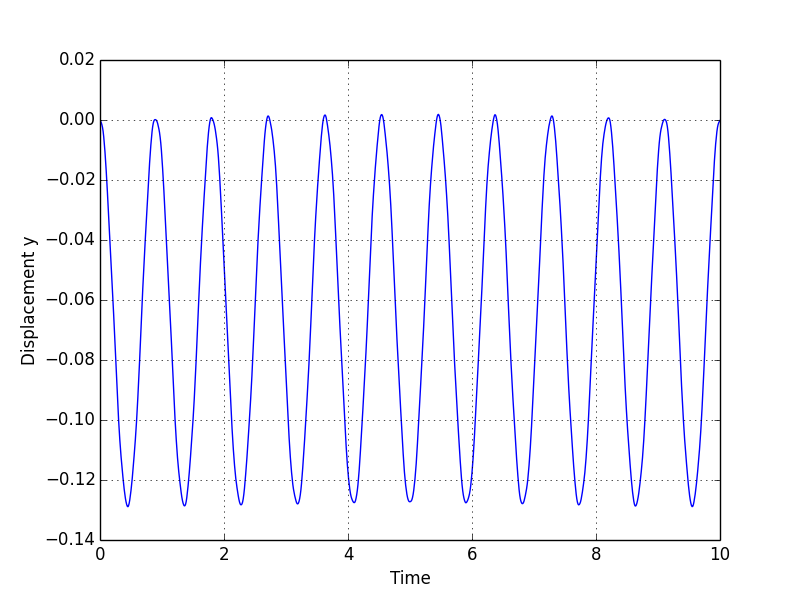
\includegraphics[width=.75\linewidth]{./Verification_Validation//Hron_Turek/dis_y.png} 
    \caption{Discplacement y} 
    \vspace{4ex}
  \end{minipage} 
  \begin{minipage}[b]{0.5\linewidth}
    \centering
    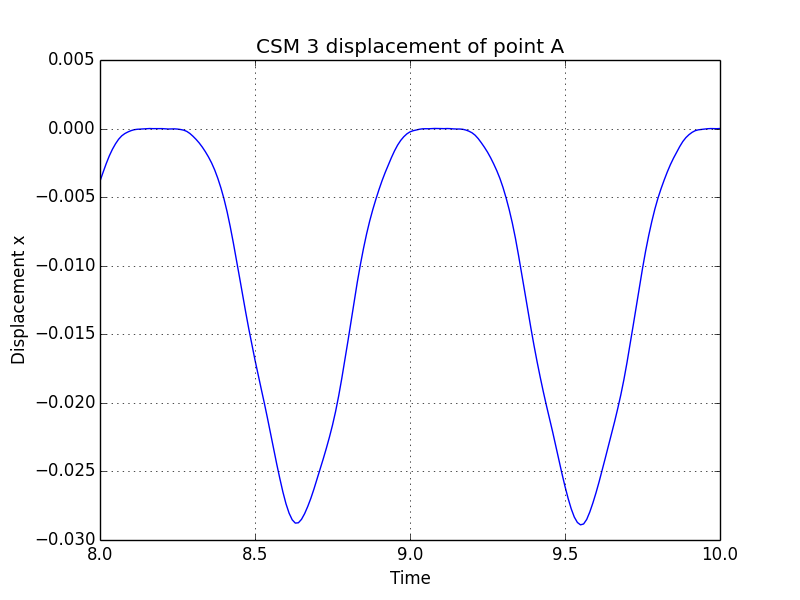
\includegraphics[width=.75\linewidth]{./Verification_Validation//Hron_Turek/dis_x_short.png} 
    \caption{Displacement x} 
    \vspace{4ex}
  \end{minipage}%% 
  \begin{minipage}[b]{0.5\linewidth}
    \centering
    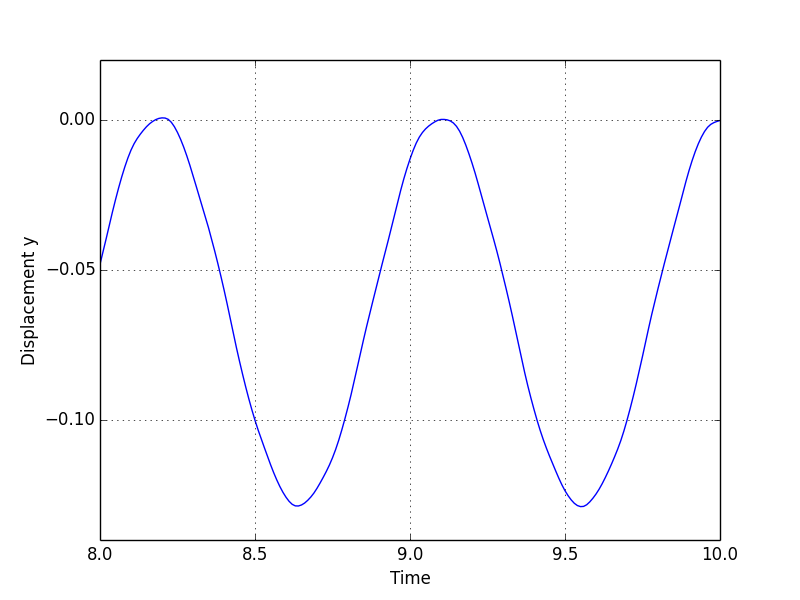
\includegraphics[width=.75\linewidth]{./Verification_Validation/Hron_Turek/dis_y_short.png} 
    \caption{Discplacement y} 
    \vspace{4ex}
  \end{minipage} 
\end{figure}

The plots \ref{CSM3_plots} is a plot of the CSM3 test. This was run with Crank-Nicholson, $\theta = 0.5$ and as we can see the energy has been preserved. 

\subsubsection*{FSI test}
Lastly we run the full FSI problem. Here we can see in \ref{fig:fluid_structure} that now both fluid and structure has a mesh. The tests are run with 2 different inflows. FSI1 gives a steady state solution while the others are unsteady. FSI-2 gives the largest deformation is therefore considered the most difficult of the three \cite{Richter2013}. The FSI-3 test has the highest inflow speed giving more rapid oscillations.

\begin{figure}[H]
\label{fig:fluid_structure}
\caption{Fluid and Structure mesh with 2698 Cells}
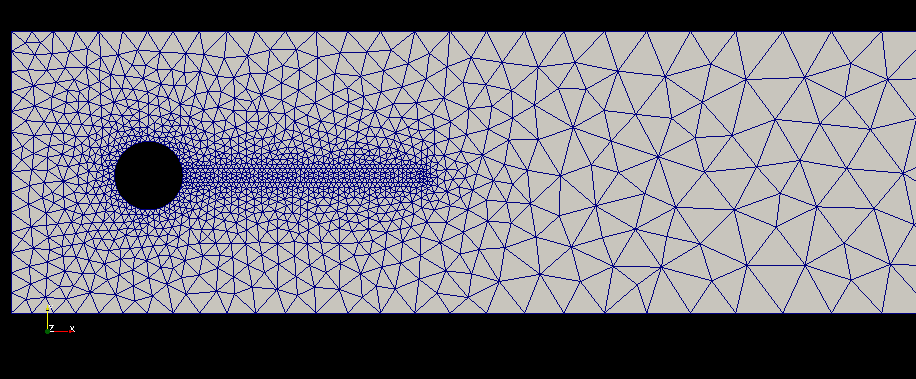
\includegraphics[scale=0.45, trim={4mm 21mm 2mm 10mm},clip]{./Verification_Validation/Hron_Turek/fluid_structure.png}
\end{figure}

\begin{table}[h!]
\centering
\caption{FSI Parameters}
\label{my-label}
\begin{tabular}{|l|l|l|l|}
\hline
Parameters & FSI1 & FSI2 & FSI3 \\ \hline
$\rho_f[10^3 \frac{kg}{m^3}]$ & 1 & 1 & 1 \\ \hline
$\nu_f [10^{-3} \frac{m^2}{s}]$ & 1 & 1 & 1 \\ \hline
$u_0$ & 0.2 & 1 & 2 \\ \hline
Re = $\frac{U d}{\nu_f}$ & 20 & 100 & 200 \\ \hline
$\rho_s[10^3 \frac{kg}{m^3}]$ & 1 & 10 & 1 \\ \hline
$\nu_s$ & 0.4 & 0.4 & 0.4 \\ \hline
$\mu_s[10^6 \frac{m^2}{s}]$ & 0.5 & 0.5 & 2 \\ \hline
\end{tabular}
\end{table}

\subsubsection*{FSI1}
\begin{table}[H]
\centering
\caption{FSI 1}
\label{my-label}
\begin{tabular}{|l|l|l|l|l|l|l|}
\hline
Cells & Dofs & $d_x(A) [x10^{-3}]$ & $d_y(A)[x10^{-3}]$ & Drag & Lift & Spaces \\ \hline
2698 & 23563 &0.0227418 &0.799314  &  14.1735 &0.761849 & P2-P2-P1 \\ \hline
10792 & 92992  &0.0227592 & 0.80795 & 14.1853 &  0.775063 &  P2-P2-P1 \\ \hline
43168 & 369448 & 00.227566 & 0.813184 & 14.2269 & 0.771071 & P2-P2-P1 \\ \hline
\textbf{ref} & \textbf{ref} & \textbf{0.0227} & \textbf{0.8209} & \textbf{14.295} & \textbf{0.7638} & \textbf{ref} \\ \hline
\end{tabular}
\end{table}

\subsubsection*{FSI2}

The FSI-2 results were with $\Delta t = 0.01, \theta = 0.51$, biharmonic bc 1, $\alpha_u = 0.01$
\begin{table}[H]
\centering
\caption{FSI-2}
\label{my-label}
\begin{tabular}{|l|l|l|l|l|l|l|l|l|}
\hline
Cells & Dofs & $d_x(A) [x10^{-3}]$ & $d_y(A) [x10^{-3}]$ & Drag & Lift & Extrapolation & BC & $\Delta t$ \\ \hline
2698 & 23563 & $-15.17 \pm 13.35  $ & $1.13 \pm 82.5$ & $160.12 \pm 17.88$ & $0.87 \pm 259.62$ & Biharmonic & 1 & 0.01 \\ \hline
2698 & 23563 & $-14.92 \pm 13.17 $ & $1.13 \pm 81.86$ & $160.28 \pm 17.94$ & $0.65 \pm 254.07$ & Biharmonic & 2 & 0.01 \\ \hline
2698 & 23563 & $-15.10 \pm 13.32 $ & $1.16 \pm 82.46 $ & $159.53 \pm,17.44 $ & $ 0.68 \pm 259.10 $ & Harmonic & - & 0.01 \\ \hline
\textbf{ref} & \textbf{ref} & $\textbf{-14.58} \pm \textbf{12.44}$ & $\textbf{1.23} \pm \textbf{80.6}$ & $\textbf{208.83} \pm \textbf{73.75}  $ & $\textbf{0.88} \pm \textbf{234.2} $ & \textbf{ref} & \textbf{ref} & \textbf{ref} \\ \hline
\end{tabular}
\end{table}


\begin{figure}[H]
\caption{Deformation at $t =9.20 $sec  using warp by vector in paraview}
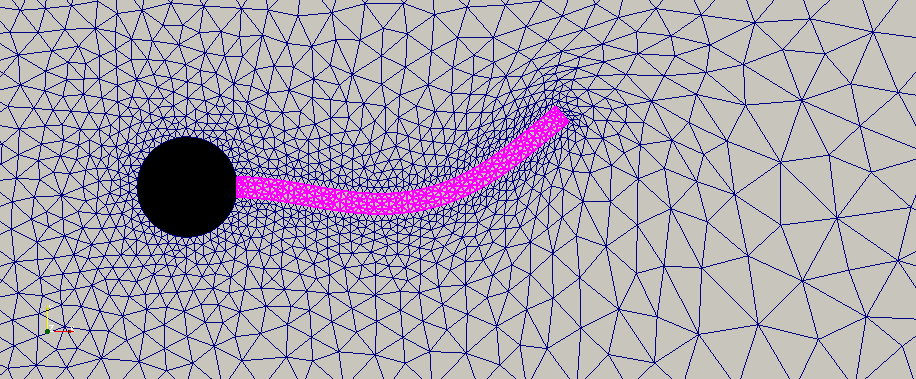
\includegraphics[scale=0.40,trim={0mm 0mm 0mm 0mm},clip]{./Verification_Validation/Hron_Turek/FSI2_d_920.png}
\end{figure}
\begin{figure}[H]
\caption{Velocity at $ t = 9.20 $sec on reference mesh}
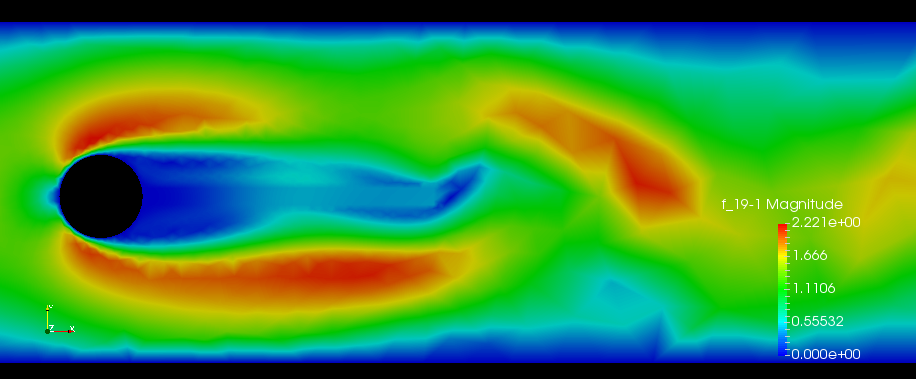
\includegraphics[scale=0.40,trim={0mm 0mm 0mm 0mm},clip]{./Verification_Validation/Hron_Turek/FSI2_u_920.png}
\end{figure}










